\documentclass{article}
\usepackage[main,final]{neurips_2025}  % NEURIPS style (neurips_2025.sty is in paper_draft/)

\usepackage[utf8]{inputenc}
\usepackage[T1]{fontenc}
\usepackage[hidelinks]{hyperref}  % REQUIRED: clickable links
\usepackage{url}
\usepackage{booktabs}  % REQUIRED: professional tables
\usepackage{graphicx}
\usepackage{amsmath,amssymb}
\usepackage{subcaption}
\usepackage{enumitem}
\usepackage{multirow}
\usepackage{algorithm}
\usepackage[noend]{algpseudocode}

% Import command files
\input{commands/math}
\input{commands/general}
%%%%% PROJECT-SPECIFIC MACROS %%%%%
% Import with: %%%%% PROJECT-SPECIFIC MACROS %%%%%
% Import with: %%%%% PROJECT-SPECIFIC MACROS %%%%%
% Import with: \input{commands/macros}

\usepackage{xspace}

%%%%%%%%%%%%%%%%%%%%%%%%%%%%%%%%%%%%%%%%%%%%%%%%%%%%%%%%%%%%%%%%%
% CONDITION / METHOD NAMES
%%%%%%%%%%%%%%%%%%%%%%%%%%%%%%%%%%%%%%%%%%%%%%%%%%%%%%%%%%%%%%%%%

\newcommand{\plain}{\textsc{Plain}\xspace}
\renewcommand{\cot}{\textsc{Generic-CoT}\xspace}  % override built-in \cot (cotangent); unused here
\newcommand{\simtom}{\textsc{SimToM}\xspace}
\newcommand{\persentence}{\textsc{Per-Sentence}\xspace}
\newcommand{\ours}{\persentence}

%%%%%%%%%%%%%%%%%%%%%%%%%%%%%%%%%%%%%%%%%%%%%%%%%%%%%%%%%%%%%%%%%
% MODEL NAMES
%%%%%%%%%%%%%%%%%%%%%%%%%%%%%%%%%%%%%%%%%%%%%%%%%%%%%%%%%%%%%%%%%

\newcommand{\gptmini}{\textsc{GPT-4.1-mini}\xspace}
\newcommand{\llama}{\textsc{Llama-3.3-70B}\xspace}
\newcommand{\claude}{\textsc{Claude-Sonnet-4.5}\xspace}
\newcommand{\gemini}{\textsc{Gemini-2.5-Flash}\xspace}

%%%%%%%%%%%%%%%%%%%%%%%%%%%%%%%%%%%%%%%%%%%%%%%%%%%%%%%%%%%%%%%%%
% DATASET NAMES
%%%%%%%%%%%%%%%%%%%%%%%%%%%%%%%%%%%%%%%%%%%%%%%%%%%%%%%%%%%%%%%%%

\newcommand{\writingprompts}{\textsc{WritingPrompts}\xspace}

%%%%%%%%%%%%%%%%%%%%%%%%%%%%%%%%%%%%%%%%%%%%%%%%%%%%%%%%%%%%%%%%%
% ABBREVIATIONS
%%%%%%%%%%%%%%%%%%%%%%%%%%%%%%%%%%%%%%%%%%%%%%%%%%%%%%%%%%%%%%%%%

\newcommand{\ie}{i.e.,\xspace}
\newcommand{\eg}{e.g.,\xspace}
\newcommand{\cf}{cf.\xspace}
\newcommand{\tom}{ToM\xspace}


\usepackage{xspace}

%%%%%%%%%%%%%%%%%%%%%%%%%%%%%%%%%%%%%%%%%%%%%%%%%%%%%%%%%%%%%%%%%
% CONDITION / METHOD NAMES
%%%%%%%%%%%%%%%%%%%%%%%%%%%%%%%%%%%%%%%%%%%%%%%%%%%%%%%%%%%%%%%%%

\newcommand{\plain}{\textsc{Plain}\xspace}
\renewcommand{\cot}{\textsc{Generic-CoT}\xspace}  % override built-in \cot (cotangent); unused here
\newcommand{\simtom}{\textsc{SimToM}\xspace}
\newcommand{\persentence}{\textsc{Per-Sentence}\xspace}
\newcommand{\ours}{\persentence}

%%%%%%%%%%%%%%%%%%%%%%%%%%%%%%%%%%%%%%%%%%%%%%%%%%%%%%%%%%%%%%%%%
% MODEL NAMES
%%%%%%%%%%%%%%%%%%%%%%%%%%%%%%%%%%%%%%%%%%%%%%%%%%%%%%%%%%%%%%%%%

\newcommand{\gptmini}{\textsc{GPT-4.1-mini}\xspace}
\newcommand{\llama}{\textsc{Llama-3.3-70B}\xspace}
\newcommand{\claude}{\textsc{Claude-Sonnet-4.5}\xspace}
\newcommand{\gemini}{\textsc{Gemini-2.5-Flash}\xspace}

%%%%%%%%%%%%%%%%%%%%%%%%%%%%%%%%%%%%%%%%%%%%%%%%%%%%%%%%%%%%%%%%%
% DATASET NAMES
%%%%%%%%%%%%%%%%%%%%%%%%%%%%%%%%%%%%%%%%%%%%%%%%%%%%%%%%%%%%%%%%%

\newcommand{\writingprompts}{\textsc{WritingPrompts}\xspace}

%%%%%%%%%%%%%%%%%%%%%%%%%%%%%%%%%%%%%%%%%%%%%%%%%%%%%%%%%%%%%%%%%
% ABBREVIATIONS
%%%%%%%%%%%%%%%%%%%%%%%%%%%%%%%%%%%%%%%%%%%%%%%%%%%%%%%%%%%%%%%%%

\newcommand{\ie}{i.e.,\xspace}
\newcommand{\eg}{e.g.,\xspace}
\newcommand{\cf}{cf.\xspace}
\newcommand{\tom}{ToM\xspace}


\usepackage{xspace}

%%%%%%%%%%%%%%%%%%%%%%%%%%%%%%%%%%%%%%%%%%%%%%%%%%%%%%%%%%%%%%%%%
% CONDITION / METHOD NAMES
%%%%%%%%%%%%%%%%%%%%%%%%%%%%%%%%%%%%%%%%%%%%%%%%%%%%%%%%%%%%%%%%%

\newcommand{\plain}{\textsc{Plain}\xspace}
\renewcommand{\cot}{\textsc{Generic-CoT}\xspace}  % override built-in \cot (cotangent); unused here
\newcommand{\simtom}{\textsc{SimToM}\xspace}
\newcommand{\persentence}{\textsc{Per-Sentence}\xspace}
\newcommand{\ours}{\persentence}

%%%%%%%%%%%%%%%%%%%%%%%%%%%%%%%%%%%%%%%%%%%%%%%%%%%%%%%%%%%%%%%%%
% MODEL NAMES
%%%%%%%%%%%%%%%%%%%%%%%%%%%%%%%%%%%%%%%%%%%%%%%%%%%%%%%%%%%%%%%%%

\newcommand{\gptmini}{\textsc{GPT-4.1-mini}\xspace}
\newcommand{\llama}{\textsc{Llama-3.3-70B}\xspace}
\newcommand{\claude}{\textsc{Claude-Sonnet-4.5}\xspace}
\newcommand{\gemini}{\textsc{Gemini-2.5-Flash}\xspace}

%%%%%%%%%%%%%%%%%%%%%%%%%%%%%%%%%%%%%%%%%%%%%%%%%%%%%%%%%%%%%%%%%
% DATASET NAMES
%%%%%%%%%%%%%%%%%%%%%%%%%%%%%%%%%%%%%%%%%%%%%%%%%%%%%%%%%%%%%%%%%

\newcommand{\writingprompts}{\textsc{WritingPrompts}\xspace}

%%%%%%%%%%%%%%%%%%%%%%%%%%%%%%%%%%%%%%%%%%%%%%%%%%%%%%%%%%%%%%%%%
% ABBREVIATIONS
%%%%%%%%%%%%%%%%%%%%%%%%%%%%%%%%%%%%%%%%%%%%%%%%%%%%%%%%%%%%%%%%%

\newcommand{\ie}{i.e.,\xspace}
\newcommand{\eg}{e.g.,\xspace}
\newcommand{\cf}{cf.\xspace}
\newcommand{\tom}{ToM\xspace}


\captionsetup[table]{aboveskip=4pt,belowskip=4pt}
\captionsetup[figure]{aboveskip=4pt,belowskip=4pt}

\bibliographystyle{plainnat}

\title{Think About the Reader Once, Not Every Sentence:\\
Per-Sentence Audience Simulation in Chain-of-Thought Hurts LLM Writing}

\author{Ari Holtzman and NeuriCo}

\begin{document}

\maketitle

\begin{abstract}
Large language models often write in a fluent-but-generic voice, as if pitched at no one in
particular. A natural explanation is that they model the reader too weakly, and a natural fix is
to force the model to simulate the reader inside its own chain-of-thought---roughly once per
sentence---so that every next sentence is chosen against a fresh prediction of how the reader
reacts. We give this hypothesis its first direct test. We generate 60 audience-targeted writing
tasks under four conditions---plain generation, generic step-by-step reasoning (a token-matched
control), one-shot audience modeling (\simtom), and the proposed per-sentence audience
simulation---and evaluate them with two separate, cross-family judge models: one role-plays the
target reader to rate audience fit, the other scores overall writing quality via blind,
order-balanced pairwise comparison. Across paired significance tests, effect sizes, and
Holm correction, the specific hypothesis is refuted while its underlying intuition is vindicated.
Modeling the reader does help: a single rich audience model written once up front is the best
condition on every metric---audience fit, engagement, genuine audience adaptation, and prose
diversity---at lower cost. Per-sentence simulation is the worst or near-worst condition: it loses
pairwise on overall quality to all three baselines (win-rates $0.08$--$0.25$, all $p < 0.001$),
adapts \emph{less} to the reader rather than more, does not reduce homogenization, and is the
longest and most token-expensive. The result replicates across two generator families. The
lesson is about granularity: think about the reader once, deeply---not reactively, sentence by
sentence.

\end{abstract}

\section{Introduction}
\label{sec:intro}

Large language models write fluently, yet their prose is often flat and generic---polished
sentences that read as if written for no one in particular. A common diagnosis is that the model
fails to model its reader: it produces text that is locally correct but pitched at a default,
average audience rather than the specific person who will read it. If this diagnosis is right,
there is an appealing, cheap fix. Rather than fine-tune the model, we could simply ask it, in its
chain-of-thought, to \emph{simulate the reader}---and to do so continuously, roughly once per
sentence, so that each next sentence is chosen against a fresh prediction of how the reader is
reacting: confused, bored, skeptical, or curious. This is an inference-time, prompt-only
intervention that anyone could apply. \emph{Does it work?}

\para{Why this matters.} Writing quality is a pervasive, high-value problem for LLMs used as
assistants, tutors, and technical communicators. If verbalizing an incremental,
per-sentence audience simulation genuinely improved writing, it would be an unusually cheap win:
no training, no reward model, no external listener---just a better prompt. The intuition also has
strong roots. The pragmatics literature shows that speakers who model their listener communicate
more successfully~\citep{andreas2016reasoning,fried2023pragmatics,takmaz2023speaking}, and the
Theory of Mind (\tom) literature shows that default LLM social reasoning is
brittle~\citep{ullman2023large,shapira2023clever}, suggesting that an explicit modeling step might
help.

\para{The gap.} Despite this, the exact intervention has never been tested for writing. Every
prior audience-aware method places the audience model \emph{outside} the generator's own
reasoning: a decode-time gradient~\citep{takmaz2023speaking}, a rerank by a separately trained
listener~\citep{andreas2016reasoning,coderesa2025}, an external
reward~\citep{styleinfusion2023}, or a formal belief update~\citep{crsa2025}. Per-sentence
mental-state simulation \emph{inside} natural-language chain-of-thought exists only for
comprehension QA and dialogue~\citep{perceptom2024,thoughttracing2025,tomagent2025}, never for
open-ended writing quality. Meanwhile, \citet{chakrabarty2025aislop} show that generic reasoning
does \emph{not} improve writing quality---so a gain from an \emph{audience-specific}
chain-of-thought would be a genuinely non-trivial result, and any claimed gain must be isolated
from ``more thinking tokens.''

\para{Our approach.} We run the first direct test of the intervention (\secref{sec:method}). We
build 60 audience-targeted writing tasks---explaining a concept to an 8-year-old, a non-technical
executive, a PhD expert, or a skeptic, plus creative stories with an assigned readership---and
generate each under four conditions that differ \emph{only} in how the model reasons about the
reader: \plain (write directly), \cot (generic ``think step by step,'' a token-matched control),
\simtom (describe the reader once, then write), and \persentence (the intervention: plan
sentence by sentence, and after each sentence simulate how this reader reacts, then choose the
next). Every condition is told exactly who the reader is, so any difference is attributable to
the \emph{reasoning strategy}, not to privileged audience information. We judge only clean final
text with two separate, cross-family models---one role-playing the reader for audience fit, one
scoring overall quality by blind pairwise comparison---and add an adaptation-gap control that
measures whether a method \emph{actually uses} the audience rather than just writing well in
general.

\para{What we find.} The specific hypothesis is refuted, but its underlying intuition is
vindicated. Audience modeling does help---but a single, rich audience model written once up front
(\simtom) is the clear winner on every metric, at lower cost. The proposed per-sentence
simulation is the worst or near-worst condition: it loses pairwise on overall quality to
\emph{all three} baselines (win-rates $0.083$--$0.250$, all $p<0.001$ after Holm correction),
scores lowest on engagement and audience fit, shows \emph{no} better audience adaptation (in fact
the smallest adaptation gap, $6.04$ vs.\ \simtom's $7.00$), does not reduce homogenization, and
is the longest ($170$ words vs.\ $147$) and most token-expensive condition. The ordering
replicates with a completely different generator (\llama). The takeaway is blunt: \emph{``think
about the reader'' helps writing; ``re-simulate the reader every sentence'' hurts it.}

\para{Contributions.}
\begin{itemize}[leftmargin=*,itemsep=0pt,topsep=0pt]
    \item We give the first direct, controlled test of per-sentence audience simulation in
    chain-of-thought for open-ended writing, isolating it from a token-matched generic-reasoning
    control and from privileged audience information.
    \item We show the intervention \emph{backfires}: it loses on overall quality to plain
    generation, generic reasoning, and one-shot audience modeling, and---via an adaptation-gap
    control---adapts to the reader \emph{less}, not more, than a one-shot audience model.
    \item We show the intuition behind it is nonetheless correct: one-shot audience modeling
    (\simtom) is the best condition on audience fit, engagement, adaptation, and diversity, at
    lower token cost, identifying \emph{granularity} as the key design axis.
    \item We replicate the full ordering across two generator families and release all $3{,}876$
    cached generations and judgments for reproducibility.
\end{itemize}

\para{Organization.} \secref{sec:related} positions our work in pragmatics, \tom, and
writing-quality research. \secref{sec:method} describes the tasks, conditions, models, and
metrics. \secref{sec:results} reports the main comparison, the adaptation-gap control,
homogenization and cost, and the cross-family replication. \secref{sec:discussion} interprets
\emph{why} per-sentence simulation hurts and discusses limitations, and \secref{sec:conclusion}
concludes.

\section{Related Work}
\label{sec:related}

\para{Audience-aware generation and pragmatics.} The Rational Speech Acts tradition models a
speaker who chooses each utterance by simulating how a listener will interpret it relative to
alternatives~\citep{andreas2016reasoning,fried2023pragmatics}. \citet{andreas2016reasoning} sample
candidate descriptions and rerank them with a simulated listener, gaining accuracy while a small
fluency weight keeps language natural; notably, the reranking reasoning did not distill into a
feedforward network, suggesting explicit inference-time reasoning matters. \citet{takmaz2023speaking}
steer a frozen speaker at decode time with a listener simulator, and find that modeling a
\emph{specific} reader (audience-aware) beats modeling a generic one (self-aware), which beats no
modeling at all. \citet{coderesa2025} reverse-generate what an audience thinks a program does and
rerank for distinctiveness, and \citet{crsa2025} maintain a formal per-turn belief over a
listener's private state, gaining most when that belief is genuinely uncertain.
\citet{styleinfusion2023} treat audience preference as an external reward. Across all of these,
audience modeling lives \emph{outside} the generator's own reasoning---as a gradient, a reranker,
a reward, or a belief-update module. Unlike these methods, we place audience modeling
\emph{inside} the generator's natural-language chain-of-thought, and ask whether doing so
per-sentence improves open-ended prose.

\para{Per-sentence and reflective mental-state simulation.} A separate line applies incremental
mental-state reasoning inside the model's own text. \citet{perceptom2024} prompt the model, per
sentence, for who perceived each piece of content, filter to the target's perspective, and then
answer, yielding large false-belief gains. \citet{thoughttracing2025} trace mental states with an
incremental, hypothesis-driven agent, and \citet{tomagent2025} infer a partner's
belief-desire-intention, predict their reply, and reflect. These are the closest method analogs to
our intervention, but all target \emph{comprehension QA or dialogue}, where the goal is to answer
a question about a mind, not to \emph{write well}. We port the per-sentence template to writing and
find that what helps comprehension hurts prose.

\para{Theory of Mind in LLMs, and the chain-of-thought caution.} Default LLM \tom is real but
brittle, collapsing under trivial adversarial perturbations~\citep{ullman2023large,
shapira2023clever}. Crucially, \citet{shapira2023clever} warn that chain-of-thought can inflate
\tom scores through leaked task structure and shortcuts, so a positive result from an
audience-simulation prompt must be checked against controls and a separate judge rather than taken
at face value. Perspective-taking prompts such as \simtom already help \tom
QA~\citep{tomsurvey2025}, and pragmatic competence grows across training
stages~\citep{altprag2025}. We heed the caution directly: we judge only clean extracted text with
judges in different families from the generator, and add an adaptation-gap control that rules out a
generic-quality confound.

\para{Writing quality and homogenization.} LLM prose is fluent but homogenized, and strong judges
struggle to separate good writing from bad~\citep{homogenization2026}. Most relevant to us,
\citet{chakrabarty2025aislop} show that generic chain-of-thought and reasoning models do
\emph{not} improve writing quality, while span-level self-editing does. This makes our question
sharp: if audience-specific reasoning helped writing, it would be a non-trivial exception to the
``more reasoning does not help writing'' finding. Building on their testbed and the homogenization
metrics of \citet{homogenization2026}, we measure quality, audience fit, adaptation, diversity,
and cost together. Our result extends theirs: even audience-specific reasoning fails to help when
applied at fine (per-sentence) granularity, whereas a coarse one-shot audience model does help.

\section{Methodology}
\label{sec:method}

\para{Research question and hypotheses.} We ask whether having an LLM simulate the target reader
in its chain-of-thought roughly once per sentence produces writing that is (i) better fit to that
reader, (ii) higher in overall quality, and (iii) more genuinely adapted to the reader, compared
to plain generation, a token-matched generic reasoning control, and one-shot audience modeling. We
decompose this into five pre-registered hypotheses: \textbf{H1} (audience fit): \persentence
beats all baselines on a separate reader model's fit rating; \textbf{H2} (quality): \persentence
beats baselines on a cross-family quality judge; \textbf{H3} (adaptation): \persentence shows the
largest audience-adaptation gap; \textbf{H4} (not just tokens): \persentence beats generic
reasoning despite both adding thinking tokens; \textbf{H5} (diversity/cost): \persentence reduces
generic sameness at acceptable cost. The independent variable is the generation \emph{condition};
dependent variables are audience-fit score, pairwise quality win-rate, adaptation gap, diversity
metrics, and length/token cost.

\subsection{Task set}

We use \textbf{audience-targeted writing}, the sharpest test of audience modeling, comprising 60
tasks. \textbf{48 explanatory} tasks pair a concept with a specific reader: ``Explain
\{concept\} for \{audience\}'' in roughly 150 words. Twelve concepts span science, finance, and
technology (vaccines, compound interest, black holes, how an LLM generates text, antibiotic
resistance, blockchain, seasons, mRNA, the stock market, encryption, photosynthesis, greenhouse
warming), crossed with four audiences that vary in expertise and disposition: \textbf{an
8-year-old child}, \textbf{a non-technical executive}, \textbf{a PhD-level expert}, and \textbf{a
skeptic who distrusts the topic}. \textbf{12 creative} tasks draw prompts from
\writingprompts~\citep{fan2018writingprompts} with an assigned target readership, for breadth.

\subsection{Conditions}

The only manipulation is \emph{how the model reasons about the reader}; crucially, every
condition is given identical information about who the reader is, so any difference is
attributable to the reasoning strategy rather than to privileged audience information. Generation
uses a clean two-step protocol---a reasoning turn, then a ``write ONLY the final piece'' turn---so
the judged text never contains chain-of-thought scaffolding.

\begin{itemize}[leftmargin=*,itemsep=1pt,topsep=2pt]
    \item \plain: no reasoning turn---write directly (the ``annoying'' egocentric default).
    \item \cot: ``think step by step to make it excellent'' (generic reasoning;
    \textbf{token-matched control} that isolates audience simulation from added
    thinking tokens).
    \item \simtom: describe the reader once (background, knowledge, what they care about, tone),
    then write.
    \item \persentence \textit{(intervention)}: plan sentence by sentence; after each sentence,
    simulate how \emph{this reader} reacts (confused, bored, skeptical, curious), then choose the
    next sentence.
\end{itemize}

\subsection{Models}

We deliberately keep the generator and both judges in \textbf{different model families} to avoid
self-preference and shortcut inflation~\citep{shapira2023clever}. The \textbf{generator} is
\gptmini (primary) with \llama for replication. The \textbf{quality judge} is \claude, used for
blind, order-balanced pairwise comparison. The \textbf{audience/listener model} is \gemini, which
\emph{role-plays the target reader} to give absolute fit, understanding, and engagement ratings
($1$--$10$) and pairwise ``which serves this reader better'' judgments, following communication-based
evaluation~\citep{fried2023pragmatics}. All calls run through OpenRouter with a fixed seed of 42.

\subsection{Evaluation metrics}

\begin{enumerate}[leftmargin=*,itemsep=1pt,topsep=2pt]
    \item \textbf{Audience fit / understanding / engagement}: the audience model, role-playing the
    reader, rates each piece $1$--$10$.
    \item \textbf{Overall writing quality}: the cross-family judge compares pairs blind, in both
    orders, controlling for position bias; we report win-rate (0.5 = tie).
    \item \textbf{Adaptation gap} (the H3 control): each concept is written for a \emph{child} and
    for an \emph{expert}; both readers rate both pieces. The gap is $\text{matched} -
    \text{crossed}$ fit. A method that truly tailors to the reader scores high for its intended
    reader and low for the other, yielding a large gap; a generic-quality method yields a gap near
    zero. This isolates real audience use from a generic quality boost.
    \item \textbf{Homogenization}: distinct-2 and self-BLEU computed within each condition.
    \item \textbf{Cost}: output length in words and reasoning (``thinking'') characters.
\end{enumerate}

\subsection{Protocol and reproducibility}

Generation uses temperature $0.7$; judging uses temperature $0.0$; the seed is $42$ throughout.
Every model call is disk-cached by a hash of (model, messages, params), so the pipeline is fully
reproducible and re-runs are free. In total we ran $240$ primary generations, $192$ replication
generations, and roughly $1{,}400$ judge calls, yielding $3{,}876$ cached responses at an estimated
API cost of \$8--15. For statistics we use paired designs across tasks: Wilcoxon signed-rank tests
on paired differences, bootstrap $95\%$ confidence intervals for win-rates (against a null of
$0.5$) and mean differences, Cohen's $d$ / rank-biserial effect sizes, and
Holm--Bonferroni correction~\citep{holm1979simple} across the multiple condition comparisons, at
$\alpha = 0.05$. An initial marker-based text extractor leaked audience-analysis preamble into
about $23\%$ of \simtom pieces; we replaced it with the two-step protocol (zero leaks) and re-ran
everything, so all reported numbers come from the clean pipeline.

\section{Results}
\label{sec:results}

We organize results around the five hypotheses. Across the board, the intervention fails: it is
near the bottom on absolute ratings (\secref{sec:res-absolute}), loses every pairwise comparison
on overall quality (\secref{sec:res-pairwise}), adapts to the reader \emph{least}
(\secref{sec:res-adapt}), and is the most homogenized and most expensive condition
(\secref{sec:res-cost}). The ordering replicates with a second generator
(\secref{sec:res-replication}). Throughout, \simtom---a one-shot audience model---is the best
condition.

\subsection{Absolute audience ratings (H1)}
\label{sec:res-absolute}

\Tabref{tab:absolute} reports the audience model's ratings while role-playing the reader.
\persentence is near the bottom on every dimension, barely above \plain and clearly below both
\cot and \simtom. Paired Wilcoxon tests (intervention vs.\ each baseline), Holm-corrected, show
\persentence is significantly \emph{worse} than \simtom on fit ($p=0.0001$), engagement
($p=0.0002$), and understanding ($p=0.057$), and worse than \cot on fit ($p=0.0007$) and
engagement ($p=0.0025$); it is statistically indistinguishable from \plain. The proposed
intervention thus fails to improve audience fit---\textbf{H1 is refuted}
(\figref{fig:absolute}).

\begin{table}[t]
\centering
\caption{Absolute audience ratings (\gemini role-playing the reader, $1$--$10$; $n=60$; higher is
better). \persentence, the intervention, is near the bottom on every dimension---below both
reasoning baselines and only marginally above \plain. \simtom is best throughout. Best results in
\textbf{bold}.}
\label{tab:absolute}
\begin{tabular}{@{}lcccc@{}}
\toprule
\textbf{Metric} & \plain & \cot & \simtom & \persentence \textit{(ours)} \\
\midrule
Audience-fit   & 6.37 & 7.12 & \textbf{7.28} & 6.52 \\
Engagement     & 5.80 & 6.45 & \textbf{6.62} & 5.93 \\
Understanding  & 9.15 & 9.30 & \textbf{9.32} & 9.08 \\
\bottomrule
\end{tabular}
\end{table}

\begin{figure}[t]
\centering
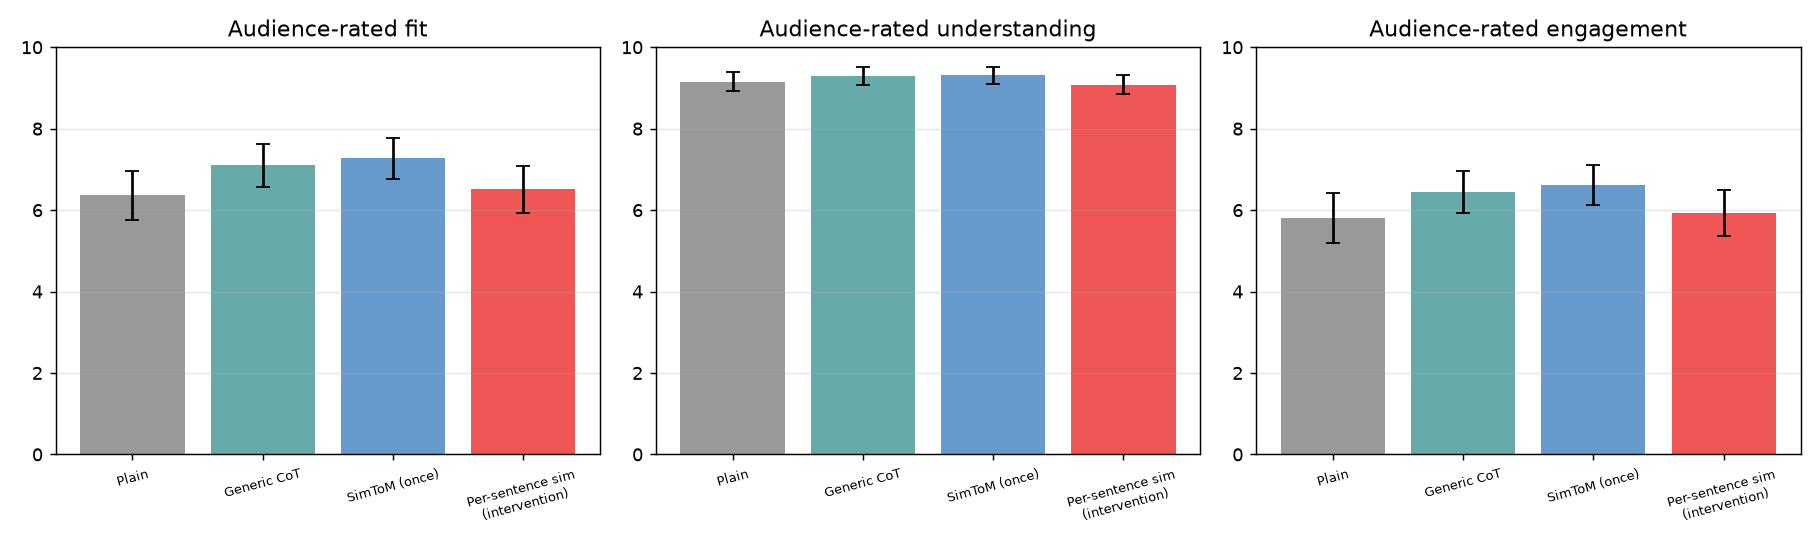
\includegraphics[width=0.6\linewidth]{figures/fig1_absolute_ratings.png}
\caption{Absolute audience ratings with $95\%$ confidence intervals. The intervention
(\persentence) sits near \plain and below both \cot and \simtom on audience fit, engagement, and
understanding; the one-shot audience model \simtom is highest on all three.}
\label{fig:absolute}
\end{figure}

\subsection{Pairwise quality and fit (H2, H4)}
\label{sec:res-pairwise}

\Tabref{tab:pairwise} reports blind, order-balanced pairwise win-rates for the intervention against
each baseline. On \textbf{overall quality} the intervention loses to all three baselines---most
heavily to \simtom, winning only $8.3\%$ of comparisons---and on \textbf{audience fit} it loses to
\cot and \simtom while merely tying \plain. All effects survive Holm correction. Because
\persentence loses to the token-matched \cot control despite both adding reasoning tokens, the
failure is not explained by ``more thinking''---\textbf{H2 and H4 are both refuted}
(\figref{fig:pairwise}).

\begin{table}[t]
\centering
\caption{Pairwise win-rate of \persentence \emph{vs.} each baseline ($n=60$; both orders averaged;
$0.5$ = tie; lower means the intervention loses more often). The intervention loses on overall
quality to \emph{all three} baselines and on audience fit to the two stronger baselines. All
significant win-rates in \textbf{bold}.}
\label{tab:pairwise}
\resizebox{\textwidth}{!}{%
\begin{tabular}{@{}lcc@{}}
\toprule
\textbf{Comparison} & \textbf{Overall quality} (\claude) & \textbf{Audience-fit} (\gemini) \\
\midrule
\persentence vs.\ \plain  & \textbf{0.250} {\scriptsize ($p<0.001$)} & 0.475 {\scriptsize ($p=0.67$, tie)} \\
\persentence vs.\ \cot    & \textbf{0.150} {\scriptsize ($p<0.001$)} & \textbf{0.250} {\scriptsize ($p<0.001$)} \\
\persentence vs.\ \simtom & \textbf{0.083} {\scriptsize ($p<0.001$)} & \textbf{0.200} {\scriptsize ($p<0.001$)} \\
\bottomrule
\end{tabular}%
}
\end{table}

\begin{figure}[t]
\centering
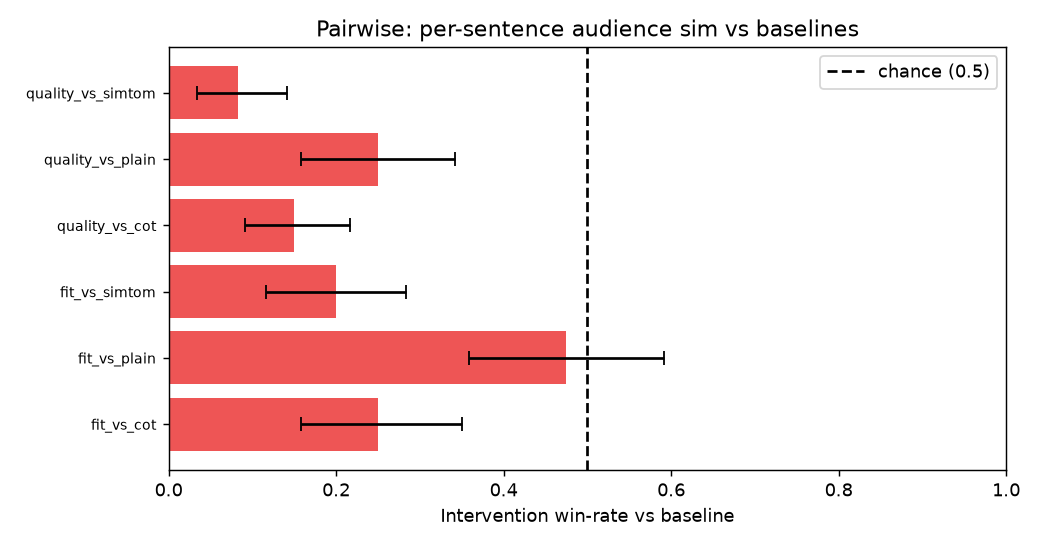
\includegraphics[width=0.6\linewidth]{figures/fig2_pairwise.png}
\caption{Pairwise win-rates for \persentence against each baseline on overall quality and audience
fit. The dashed line marks $0.5$ (tie). Every bar falls below the line: the intervention loses on
quality to all baselines and on fit to \cot and \simtom.}
\label{fig:pairwise}
\end{figure}

\subsection{Does the method actually use the audience? (H3)}
\label{sec:res-adapt}

If per-sentence simulation genuinely tailored writing to the reader, it should show the
\emph{largest} adaptation gap. Instead it shows the \emph{smallest}, tied with \plain
(\Tabref{tab:adapt}). Its gap of $6.04$ is significantly smaller than \simtom's $7.00$
($\Delta=-0.96$, Cohen's $d=-1.27$, $p=0.004$ Holm-corrected) and smaller than \cot's $6.67$
($\Delta=-0.62$, $d=-0.75$). The one-shot audience model, which commits to a single coherent
stance about the reader, adapts \emph{most}. \textbf{H3 is refuted}: the intervention does not use
the audience more---it uses it less (\figref{fig:adapt}).

\begin{table}[t]
\centering
\caption{Adaptation gap (matched-reader minus crossed-reader fit; $n=12$ concepts; higher means
the method tailors more to its intended reader). \persentence has the \emph{smallest} gap,
significantly below \simtom, which has the largest. Best in \textbf{bold}.}
\label{tab:adapt}
\begin{tabular}{@{}lcccc@{}}
\toprule
& \plain & \cot & \simtom & \persentence \textit{(ours)} \\
\midrule
Adaptation gap & 6.08 & 6.67 & \textbf{7.00} & 6.04 \\
\bottomrule
\end{tabular}
\end{table}

\begin{figure}[t]
\centering
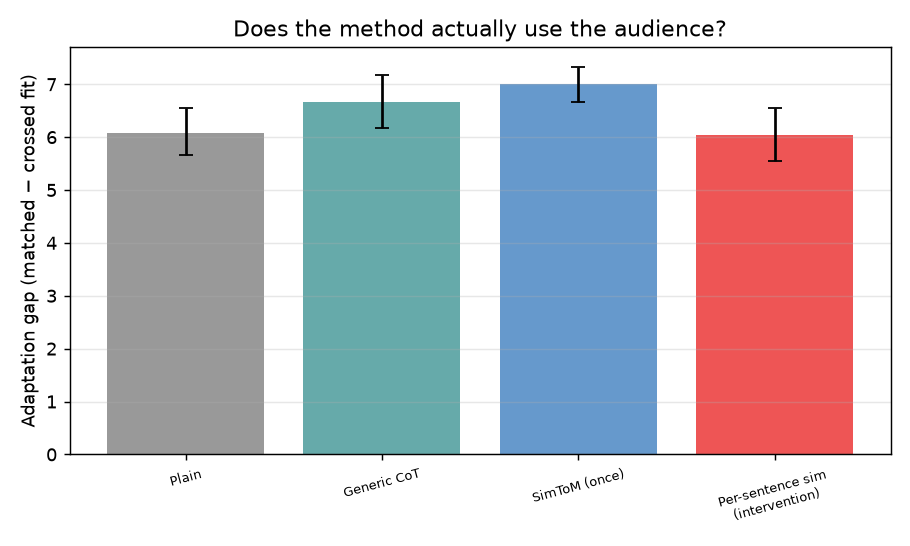
\includegraphics[width=0.6\linewidth]{figures/fig3_adaptation_gap.png}
\caption{Adaptation gap by condition. A larger gap means the method writes differently for
different readers. \persentence adapts \emph{least} (tied with \plain); \simtom adapts most,
contradicting the hypothesis that finer-grained reader simulation yields stronger adaptation.}
\label{fig:adapt}
\end{figure}

\subsection{Homogenization and cost (H5)}
\label{sec:res-cost}

\Tabref{tab:cost} reports diversity and cost. \persentence is the \emph{most} homogenized
condition (highest self-BLEU, lowest distinct-2, tied with \plain) and simultaneously the longest
($170$ words vs.\ $\sim$147) and most token-expensive (2480 thinking characters). \simtom is the
\emph{least} homogenized. So the intervention does not buy diversity with its extra tokens---it
costs the most and produces the most generic prose. \textbf{H5 is refuted}
(\figref{fig:cost}).

\begin{table}[t]
\centering
\caption{Homogenization and cost by condition ($\uparrow$/$\downarrow$ = higher/lower is better).
\persentence is the most homogenized (tied with \plain) \emph{and} the longest and most
token-expensive; \simtom is the least homogenized. Best in \textbf{bold}.}
\label{tab:cost}
\begin{tabular}{@{}lcccc@{}}
\toprule
\textbf{Condition} & distinct-2 $\uparrow$ & self-BLEU $\downarrow$ & words & thinking chars \\
\midrule
\plain        & 0.823 & 0.406 & 148 & 0 \\
\cot          & 0.842 & 0.383 & 144 & 2086 \\
\simtom       & \textbf{0.857} & \textbf{0.363} & 147 & 1762 \\
\persentence \textit{(ours)} & 0.823 & 0.402 & 170 & 2480 \\
\bottomrule
\end{tabular}
\end{table}

\begin{figure}[t]
\centering
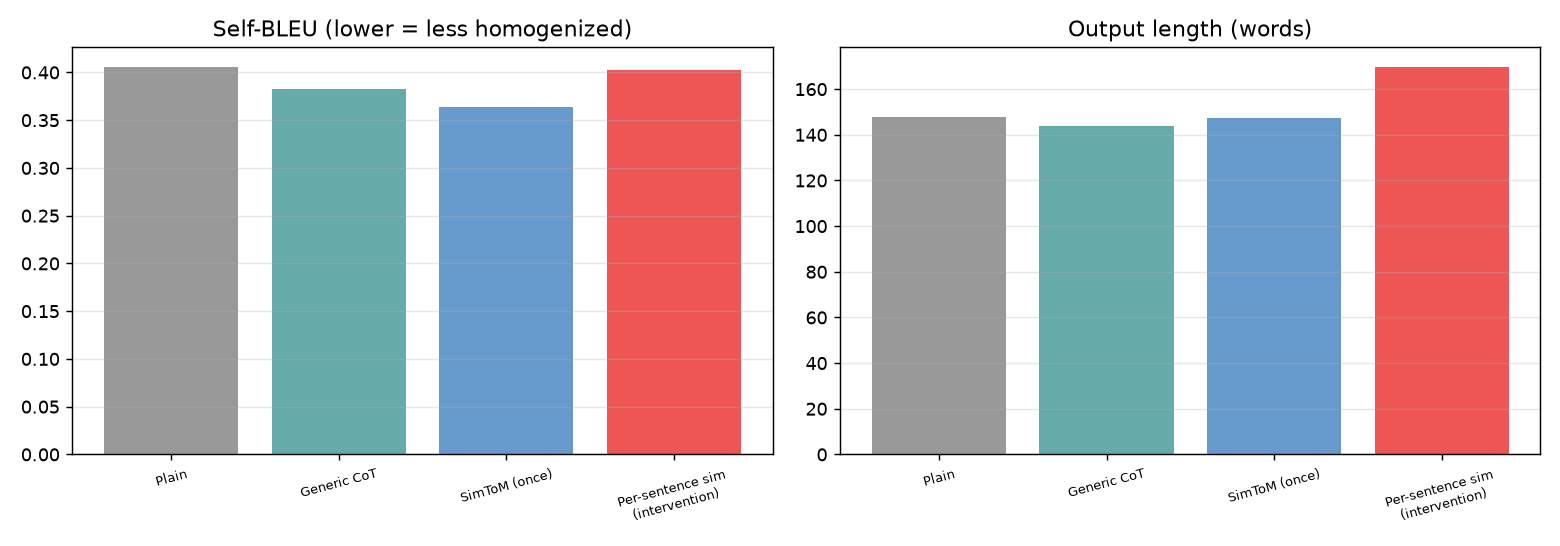
\includegraphics[width=0.6\linewidth]{figures/fig4_diversity_cost.png}
\caption{Diversity and cost. \persentence combines the worst diversity (tied with \plain) with the
highest word count and thinking-token cost, while \simtom achieves the best diversity at lower
cost.}
\label{fig:cost}
\end{figure}

\subsection{Cross-family replication (\llama)}
\label{sec:res-replication}

The same ordering holds with a completely different generator. On the 48 explanatory tasks,
\persentence is worst on fit ($5.52$ vs.\ \simtom/\cot $5.90$) and engagement ($5.02$ vs.\
\simtom $5.46$), and loses pairwise to \emph{every} baseline on both quality (win-rates
$0.115$--$0.260$) and fit (win-rates $0.167$--$0.333$), all significant. The strongest loss is
again to \simtom on quality (win-rate $0.115$, $p<10^{-8}$). The negative result is therefore not
specific to one model family.

\section{Discussion}
\label{sec:discussion}

\para{The direction of the intuition is right; the mechanism is wrong.} Audience modeling clearly
helps: both \cot and \simtom beat \plain, and \simtom---an explicit one-shot audience model---is
the best condition on \emph{every} metric, including the adaptation-gap control that specifically
measures genuine audience use. So the premise that LLMs write generically partly because they
model the reader weakly is supported. What fails is the specific proposed fix. Simulating the
reader every sentence does not just add nothing; it actively backfires, dragging the writing below
even plain generation on overall quality.

\para{Why does per-sentence simulation hurt?} Three mechanisms are visible in the outputs.
\emph{First, local reactivity destroys global craft.} Choosing each next sentence from the
reader's momentary reaction yields prose that is locally coherent but loses arc, voice, and payoff.
In one children's-story task, \simtom builds a whimsical arc with a delightful closing button
(``Death's Help Desk: Making Life Interesting Since Forever''), whereas the per-sentence version
stays plot-mechanical, keeps an adult phrase (``living forever sucks''), and drifts into heavier
themes (``watching everyone I loved grow old and leave'')---each next sentence locally reasonable,
the whole globally off-key for a child. \emph{Second, it adapts less, not more}
(\secref{sec:res-adapt}). A single rich audience model front-loads a coherent stance---``this is a
scared 8-year-old: stay warm, concrete, gentle''---that governs the entire piece, whereas
per-sentence reactions are noisier and pull the text in inconsistent directions, washing out
adaptation. \emph{Third, bloat.} The intervention runs about $15\%$ longer and spends the most
thinking tokens, yet yields worse writing---the opposite of the token-for-quality trade the
hypothesis assumed.

\para{Granularity is the key axis.} Our result directly echoes and extends
\citet{chakrabarty2025aislop}'s finding that more reasoning does not improve writing: even
\emph{audience-specific} reasoning fails to help when applied at fine (per-sentence) granularity,
while a coarse, one-shot audience model does help. The sweet spot is ``model the reader once,
richly,'' not ``re-model every sentence.'' This isolates granularity---rather than the presence or
absence of audience modeling---as the design variable that decides whether audience reasoning
helps or fragments the prose.

\para{Validity.} Several safeguards make the negative result credible. The judges are in different
families from the generators, so self-preference cannot explain the ranking; pairwise judging is
blind and order-balanced against position bias; only clean final text is judged, after a two-step
protocol eliminated a real scaffolding-leak bug we caught mid-study (\secref{sec:method}); the
adaptation-gap control rules out a generic-quality confound; and the full ordering replicates
across two generators. The effect sizes are large (win-rates as low as $0.083$) and consistent,
not marginal.

\para{Limitations.} We test a single granularity---``every sentence.'' An intermediate granularity
(per-paragraph, or once-then-one-revision-pass) might recover a benefit; we did not sweep it. Fit
and quality come from LLM judges rather than humans; although the judges are cross-family and the
effect is large and replicated, a small human evaluation would strengthen the quality claim. The
result also bounds \emph{one} careful, faithful phrasing of the per-sentence prompt, not every
conceivable one. We study short-form writing ($\sim$150 words), where global consistency is easy
to maintain without per-sentence tracking; the intervention might matter more for long documents.
Finally, our task set is 60 tasks (48 for replication); paired tests and bootstrap intervals
mitigate this, but larger, more diverse task sets would tighten the estimates.

\para{Broader implications.} For practitioners, the actionable takeaway is simple and cheap:
prompt the model to build one rich picture of the reader before writing, and do not ask it to
re-simulate the reader sentence by sentence. More broadly, the result is a caution against
importing scaffolds that help \emph{comprehension} (where per-sentence perspective tracking is
known to help~\citep{perceptom2024}) directly into \emph{generation}, where global structure is
part of the quality being measured.

\section{Conclusion}
\label{sec:conclusion}

We gave the first direct test of a natural, appealing idea: that an LLM writes better if it
simulates its reader in chain-of-thought roughly once per sentence. Across 60 audience-targeted
tasks, four conditions, two cross-family judges, an adaptation-gap control, and a replication on a
second generator, the answer is a clear \emph{no}. Per-sentence audience simulation makes writing
\emph{worse} on quality, engagement, audience fit, adaptation, and diversity, while costing the
most tokens: it loses pairwise on overall quality to plain generation, generic reasoning, and
one-shot audience modeling alike (win-rates $0.083$--$0.250$, all $p<0.001$).

\para{Key takeaway.} The deeper intuition survives: audience modeling does help writing, but its
effective form is a \emph{single, rich audience model written once up front} (\simtom), which
beats every alternative on every metric we measured, at lower cost. The lesson is about
granularity---think about the reader once, deeply, not reactively sentence by sentence. Re-modeling
the reader every sentence makes the model locally reactive and strips away the global voice, arc,
and craft that make prose good.

\para{Future work.} Four directions follow naturally. (1) A \emph{granularity sweep}---once,
per-paragraph, per-sentence---to map where audience reasoning stops helping and starts fragmenting
the prose. (2) \emph{\simtom plus one revision pass} (``re-read as the reader, fix what jars''),
likely the practical sweet spot, pairing the winning one-shot model with a single global critique.
(3) \emph{Human evaluation} on the \simtom-vs-\plain and \persentence-vs-\simtom contrasts. (4)
\emph{Long-form} documents, where the global-consistency costs of per-sentence tracking may differ.
An open question is whether per-sentence simulation's failure is fundamental---local optimization
losing global structure---or an artifact of doing it \emph{before} writing rather than as
\emph{revision}; direction (2) would distinguish these.

\para{Reproducibility.} All $3{,}876$ cached generations and judgments, the four figures, and the
summary statistics are released so the full pipeline can be re-run for free.


\bibliography{references}

\end{document}
